\documentclass{article}
\usepackage{vaibhavblayer}
\instagramp

\header{210622}{MAG}{02}[E]
\footer{3}

\begin{document}

\pagecolor{white!85!orange}
\color{white!10!purple}

\title{work done in a constant magnetic field}

\vspace*{\fill}
\begin{center}
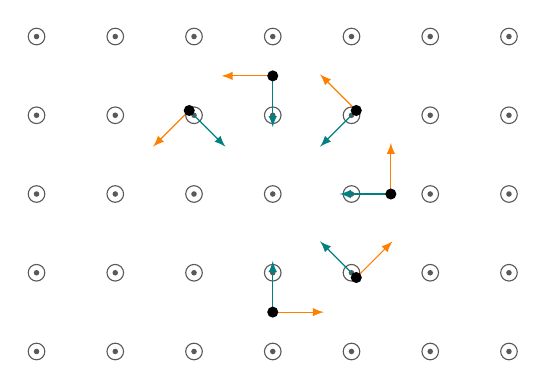
\begin{tikzpicture}
\begin{scope}[opacity=0.65]
\foreach  \x in {0,1,...,6}
   {
		\foreach  \y in {0,1,...,4}
   {
		\fill (\x, \y) circle(1pt);   
		\draw (\x, \y) circle(3pt);
   };   
   };
\end{scope}
\begin{scope}[black, >=latex, thick, xshift=3cm, yshift=0.5cm, rotate around= {0:(0, 0)}]
	
	\xangle[->]{0,1.5}{-90}{225}{1.5}[$ $];

\foreach  \a in {0,45,...,225}
   {
\begin{scope}[ thin, rotate around= {\a:(0, 1.5)}]
\coordinate (a) at (0,0);
	
		\draw[->, orange] (a) --+(0.65, 0);
	\draw[->, teal] (a)--+(0, 0.65);
\fill (a) circle(2pt);
\end{scope}	
};
\end{scope}

\end{tikzpicture}
\end{center}

\vspace*{\fill}

\begin{minipage}{2cm}
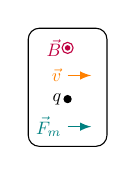
\begin{tikzpicture}
\begin{scope}[>=latex, thin, every node/.style={scale=0.65}]
\coordinate (a) at (0,0);
		\draw[->, orange] (a)++(0, 0.15) node[left]{$\vec{v}$} --+(0.3, 0);	
	\draw[->, teal] (a)++(0, -0.5) node[left]{$\vec{F}_m$}--+(0.3, 0);
\fill[black] (a)++(0, -0.15) node[left]{$q$} circle(1.5pt);

\fill[purple] (a)++(0, 0.5)  circle(1pt);
\draw[purple] (a)++(0, 0.5) node[left]{$\vec{B}$} circle(2pt);
\end{scope}
\draw[ rounded corners] (a)++(-0.5, -0.75) rectangle (0.5, 0.75);
\end{tikzpicture}
\end{minipage}
\begin{minipage}{4cm}
\[
W =\int \vec{F}_m \cdot d\vec{r} = \int q \left( \vec{v} \times \vec{B} \right) \cdot \vec{v}dt = 0
\]
\end{minipage}
\end{document}